\section{Grundbegreberne inden for IT-sikkerhed}

\subsection{Læringsmål}

\begin{itemize}
	\item Forklar de vigtigste grundbegreber indenfor IT-sikkerhed.
	\item Hvad siger lovgivning og anbefalinger/standarder om opbevaring af	passwords?
	\item Hvordan kan man selv implementere brugerautentikation?
	\item Hvilke alternativer er der til selv at implementere brugerautentikation?
\end{itemize}

\subsection{Forklar de vigtigste grundbegreber indenfor IT-sikkerhed}
Man vil beskytte \textbf{assets}, som har værdi. Det kan være: hardware, software, data, personer eller processer. Her har særlig data stor værdi, da det ikke nødvendigvis kan genskabes, ligesom hardware etc.

\subsubsection{Risikovurdering}
Når \textit{værdien} af et \textbf{asset} skal bestemmes, kan følgende tages i betragtning: menneskeliv, monetær omkostning, tab af omdømme/goodwill/rating, genskabelighed, juridiske konsekvenser (GDPR), tabt arbejdsfortjeneste etc.

\subsubsection{Fejltyper}
En systemfejl opstår på baggrund af en af to ting: 

\begin{itemize}
	\item Besign failure
	\item Malicious attack
\end{itemize}

\subsubsection{Sårbarhed, trussel og kontrol}
Forklaring af termerne:

\paragraph{Sårbarhed}
Det svageste led i kæden.

\paragraph{Trussel}
Omstændigheden som kan lede til skade.

\paragraph{Kontrol}
Handling, enhed, procedure eller teknik, som hindre trusselen i at udnytte sårbarheden.

\subsubsection{CIA triad}
Ressourceegenskaber, som en trussen kan udnytte:

\paragraph{Confidentiality}
Ressourcen må kun tilgås af autoriserede personer.

\paragraph{Integrity}
Ressourcen må kun ændres af autoriserede personer. 

\paragraph{Availability}
Autoriserede personer skal have adgang når det er nødvendigt.

\subsection{Policy}
Sættes op for at bestemme \textbf{hvem}, der kan tilgå \textbf{hvad} på hvilken \textbf{måde}. Vist på Figur~\ref{fig:policy}. 

\begin{figure}[H]
	\centering
	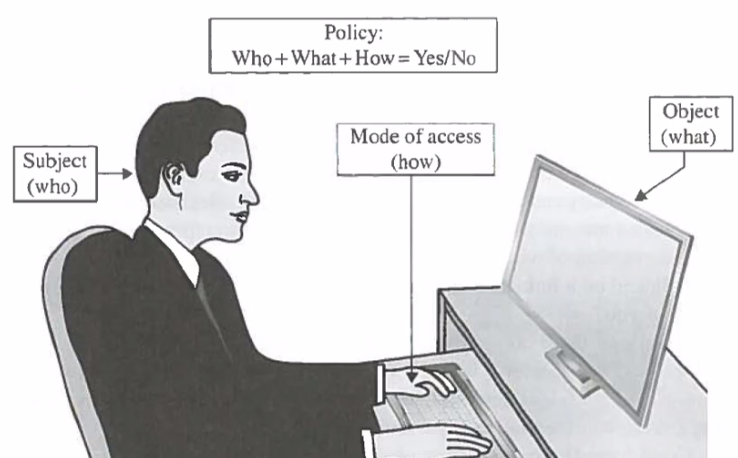
\includegraphics[width=0.8\linewidth]{figs/spm1/policy}
	\caption{Policy illustration}
	\label{fig:policy}
\end{figure}

\subsubsection{Angribere}
Alt efter typen af angriber skal der tages forskellige forholdsregler.

\begin{itemize}
	\item Individer
	\item Organisationer
	\item Regeringer
\end{itemize}

\subsection{Hvad siger lovgivning og anbefalinger/standarder om opbevaring af passwords?}

\subsubsection{Lovgivning}

\subsubsection{Opbevaring af password}
SHA256 or GTFO.

\begin{enumerate}
	\item Salt
	\item Hash
\end{enumerate}

\subsection{Hvordan kan man selv implementere brugerautentikation?}

\subsubsection{JSON web token}
Base64 encoded token, som kan valideres uden at skulle holde på et \textit{state}.

\begin{itemize}
	\item Header
	\item Payload
	\item Signature
\end{itemize}

\subsection{Hvilke alternativer er der til selv at implementere brugerautentikation?}

\begin{itemize}
	\item .NET Identity
\end{itemize}
